\documentclass[a4paper,11pt]{jsarticle}


% 数式
\usepackage{amsmath,amsfonts}
\usepackage{bm}
\usepackage{physics}
% 画像
\usepackage[dvipdfmx]{graphicx}
% ローマ数字
\usepackage{otf}
% 単位
\usepackage{siunitx}
% 表
\usepackage{multirow}
% 化学反応
\usepackage[version=4]{mhchem}


\begin{document}

\title{普遍性生物学レポート}
\author{05-211525 齋藤駿一}
\date{\today}
\maketitle

\section{はじめに}
本レポートでは,Report 2の問題について考えをまとめた.
問題は次の通りである.
\begin{quote}
  Himeoka's model demonstrated that
  including a component that interferes with
  the autocatalytic reaction can generate
  the transition to stationary and death
  phases.
  Expand this model to that with a more
  complex chemical reaction network and
  analyze how the transition can be
  characterized (e.g., statistical laws?).
\end{quote}
問題文には「定常期・死滅期への遷移」とあるが,これが行われるか否かは外部栄養濃度によって決まる.
そこで本レポートでは,姫岡モデルを拡張したときに外部栄養濃度の「休眠-死転移点」と「活性-休眠転移点」にどのような影響が及ぶかを探求した.
まず,オリジナルの姫岡モデルをPythonで実装し,転移点がどう決まるかの議論をまとめた.
次に,このモデルの拡張としてランダムな反応ネットワークを導入したものを考え,それも実装した.
最後に,この拡張した姫岡モデルの計算結果を観察した.
その結果,オリジナルの姫岡モデルを包含する反応ネットワークに対し,ほぼ同じ転移点での転移が確認できた.
しかし,本レポートではごく小さな反応ネットワークでしか計算できず,そもそも反応ネットワークによっては転移が確認できないものもあった.
ただし,最もよく成長している反応ネットワークでは二段階転移がオリジナルの姫岡モデルとほぼ同じ転移点において確認できたことから,進化計算をすることで姫岡モデルの挙動を引き出せると考えられる.

\section{姫岡モデルの概要}
\subsection{モデルの実装}
姫岡モデル\cite{himeoka}では,細胞外の栄養分死\ce{S_{ext}},細胞内の栄養分子S,正常な代謝物A,ゴミ分子B,複合体Cの4種類の分子が登場する.
それらの間で,分子Aを介した輸送
\begin{equation}
  \ce{S_{ext} <=> S}
\end{equation}
および化学反応
\begin{equation}
  \ce{S -> A},\qquad \ce{S -> B},\qquad \ce{A + B <=> C}
\end{equation}
が起こると仮定し,レート方程式を
\begin{align}
  \dv{S}{t} &= -F_A(S)A - F_B(S)A + A(S_{\mathrm{ext}}-S)-\mu S\\
  \dv{A}{t} &= F_A(S)A - G(A,B,C) - d_A A - \mu A\\
  \dv{B}{t} &= F_B(S) A - G(A,B,C) - d_B B - \mu B \\
  \dv{C}{t} &= G(A,B,C) - d_C C - \mu C
\end{align}
で与える.
ここで,$d_A,d_B,d_C$はそれぞれ分子A,B,Cの分解速度であり,$\mu=F_A(S)A$は細胞の成長速度である.
また,ここでは
\begin{equation}
  F_A(S) = \frac{vS}{K+S}\frac{S}{K_t+S},\qquad F_B(S) = \frac{vS}{K+S}\frac{K_t}{K_t+S},\qquad G(A,B,C) = k_p AB - k_m C
\end{equation}
ととることで,Sの濃度とともに反応\ce{S -> A or B}の速度が増加し,
さらに\ce{S -> B}の速度に対する\ce{S -> A}の速度の比が増加するようにする.
つまり,栄養が豊富にあるほど反応のエラー率$F_B(S)/F_A(S)$は低くなる.

このモデルを実装し,外部栄養濃度$S_{\mathrm{ext}}$と成長速度$\mu$および濃度$A$の関係を図示すると,図\ref{fig:himeoka_trans}のようになる.
図より,$S_{\mathrm{ext}}> 10^1$では$\mu,A$ともにほぼ頭打ちとなるが,$10^{-2}<S_{\mathrm{ext}}<10^1$ではどちらも数桁小さい値にとどまり,$S_{\mathrm{ext}}<10^{-2}$ではどちらもほぼゼロとなる.
これらの領域はそれぞれ,細胞の活発な状態,休眠した状態,そして死んだ状態に対応すると考えられる.

\begin{figure}[htbp]
  \centering
  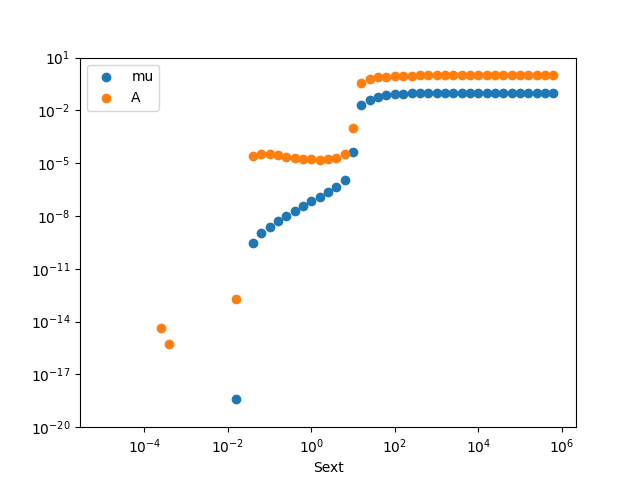
\includegraphics[width=10cm]{himeoka_trans.png}
  \caption{時刻$t=10^{12}$における,外部栄養濃度$S_{\mathrm{ext}}$に対する成長速度$\mu$および濃度$A$の関係.$S_{\mathrm{ext}}< 10^{-2}$では$\mu,A$は多くの場合$10^{-20}$に満たない微小な正または負の値をとっていた.ただし,パラメータは$v=0.1, k_p=1, k_m=10^{-6}, K=1, K_t=10, d_A=d_B=10^{-5},d_C=10^{-12}$ととり,刻み幅$dt=10^5$で計算した.初期値は$S=S_{\mathrm{ext}}, A=1, B=C=0$とした.}
  \label{fig:himeoka_trans}
\end{figure}

\subsection{転移のメカニズム}
まず,なぜ休眠-死の転移が起こるのかを考える.
複合体形成を無視($G(A,B,C)=0$を仮定)すれば,レート方程式より
\begin{equation}
  \dv{A}{t} = F_A(S)A - F_A(S)A^2 - d_A A 
\end{equation}
となる.
よって,定常状態では
\begin{equation}
  A = 0,\quad 1 - \frac{d_A}{F_A(S)} >0
\end{equation}
すなわち
\begin{equation}
  \mu = 0,\quad F_A(S)-d_A >0
\end{equation}
のいずれかが成り立つ.
そのため,$S\approx S_{\mathrm{ext}}$と考えれば,$F_A(S^{\mathrm{inact-death}}_{\mathrm{ext}})=d_A$を満たす濃度$S^{\mathrm{inact-death}}_{\mathrm{ext}}$が休眠-死転移点であり,これより低い濃度では細胞は死ぬと考えられる.
計算で用いたパラメータ$v=0.1, K=1, K_t=10, d_A=10^{-5}$を代入すると,$S^{\mathrm{inact-death}}_{\mathrm{ext}}\approx \SI{3.2e-2}{}$と求まる.
これは,図\ref{fig:himeoka_trans}で確認した休眠-死転移点と概ね一致する.

次に,活性-休眠の転移が起こる理由を考える.
$d_B\approx 0, k_m\approx 0$とすれば,レート方程式より
\begin{align}
  \dv{A}{t} &= F_A(S)A - k_p AB - F_A(S)A^2 \\
  \dv{B}{t} &= F_B(S)A - k_p AB - F_A(S)AB
\end{align}
となる.
よって,定常状態では
\begin{align}
  A &= 1 - \frac{k_p}{F_A(S)}B >0 \\
  B &= \frac{F_B(S)}{F_A(S)+k_p}
\end{align}
すなわち
\begin{equation}
  \mu = F_A(S)\left(1-\frac{k_p}{F_A(S)}\frac{F_B(S)}{F_A(S)+k_p}\right) >0
\end{equation}
が成り立つ.
つまり,
\begin{equation}
  k_p F_B(S) < F_A(S)^2 + k_p F_A(S) = \left(F_A(S) + \frac{k_p}{2}\right)^2 - \frac{k_p^2}{4}
\end{equation}
であり,これを整理すると
\begin{equation}
  1+\frac{2F_A(S)}{k_p} > \sqrt{1+\frac{4F_B(S)}{k_p}}
\end{equation}
が得られる.
そのため,$S\approx S_{\mathrm{ext}}$と考えれば,$1+\frac{2F_A(S^{\mathrm{act-inact}}_{\mathrm{ext}})}{k_p} = \sqrt{1+\frac{4F_B(S^{\mathrm{act-inact}}_{\mathrm{ext}})}{k_p}}$を満たす濃度$S^{\mathrm{act-inact}}_{\mathrm{ext}}$が活性-休眠転移点であり,これより低い濃度では細胞は休眠すると考えられる.
計算で用いたパラメータ$v=0.1, K=1, K_t=10, k_p=1$を代入すると,$S^{\mathrm{act-inact}}_{\mathrm{ext}}\approx 9.6$と求まる.
これは,図\ref{fig:himeoka_trans}で確認した活性-休眠転移点と概ね一致する.
また,以上の変形は,$k_m\approx 0$の下では$S<S^{\mathrm{act-inact}}_{\mathrm{ext}}$において細胞が死ぬことを意味する.
逆に言えば,休眠状態の存在は複合体の分解($k_m$)の恩恵であると考えることができる.


\section{姫岡モデルの拡張}
姫岡モデルはたった4変数で2つの転移が現れる興味深いモデルだが,変数や反応の数を増やしたときにこの性質がどこまで保たれるかは明らかではない.
そこで,次のような拡張を考えた.

まず,系の構成要素として,細胞外の栄養分子$\ce{S_{ext}}$,細胞内の栄養分子$\ce{S}=x_0$,$N-1$個の正常な代謝物$\ce{A_i}=x_i(i\in\{1,\cdots,N-1\})$,栄養分子および正常な代謝物$x_j(j\in\{0,1,\cdots,N-1\})$のゴミ分子$\ce{B_j}=x_{N+j}$,栄養分子および正常な代謝物$x_i(i\in\{0,1,\cdots,N-1\})$とゴミ分子$\ce{B_{j}}(j\in\{0,1,\cdots,N-1\})$の複合体$\ce{C_{i j}}=x_{2N+Ni+j}$の計$N(N+2)$種類の分子を考える.
ここで,ある$1\le M \le N-1$が与えられ,正常な代謝物のうち$x_1,\cdots,x_M$だけが成長速度に寄与すると仮定する.
また,簡単のため$x_1$のみが栄養分子の輸送に寄与すると仮定する.

加えて,ランダムに選んだ$i,j,k\in\{0,\cdots,N-1\}$の組に対し,化学反応
\begin{equation}
  x_i + x_k \ce{->} x_j + x_k,\qquad x_i + x_k \ce{->} x_{N+j} + x_k \label{reac}
\end{equation}
を仮定する.
これらの反応速度は,姫岡モデルに倣ってそれぞれ$F_A(x_i)x_k$,$F_B(x_i)x_k$とする.
ランダムな$i,j,k$の組の選び方としては,まずすべての$i,j$の組を考え,$x_i$から$x_j$を生成する反応を確率$p$で実現させ,実現する各反応に対し$k$として$\{0,\cdots,N-1\}$のどれかを等確率で選んだ.
ただし,今回は$i\neq j,\,k\neq 0$とし\footnote{$k\neq 0$とした理由は,栄養分子に触媒される反応は基本的に平衡に至らないからである.},さらに反応を反応物から生成物の向きに辿ったときに,栄養分子から成長に寄与する分子に到達する経路が見つからないような反応ネットワークは除外した.
また,ランダムに選んだ$i,j\in\{0,\cdots,N-1\}$に対し,複合体形成反応
\begin{equation}
  x_i + x_{N+j} \ce{<=>} x_{2N+Ni+j}
\end{equation}
を考える.
反応速度は$G(x_i,x_{N+j},x_{2N+Ni+j})$とする.
ただし,今回は簡単のため$i=j=0,\cdots,N-1$の$N$通りの「対角化された」複合体形成反応のみ仮定し,ランダム性は排除する.

以上より,実現するすべての反応\eqref{reac}の組$[i,j,k]$の集合$R$を用いて,レート方程式は$a,\,b\in\{0,\cdots,N-1\}$に対して
\begin{align}
  \dv{x_a}{t} &= \sum_{[i,j,k]\in R} (s_{ija}F_A(x_i)-\delta_{ia}F_B(x_i))x_k
  - \sum_{j=0}^{N-1} G(x_a,x_{N+j},x_{2N+Na+j})\notag\\
  &\qquad +\delta_{a0}x_1(S_{\mathrm{ext}}-x_0)-(\mu + d_A(1-\delta_{a0})) x_a\\
  \dv{x_{N+b}}{t} &= \sum_{[i,j,k]\in R} \delta_{ib}F_B(x_i)x_k - \sum_{i=0}^{N-1} G(x_i,x_{N+b},x_{2N+Ni+b}) -(\mu + d_B) x_{N+b}\\
  \dv{x_{2N+Na+b}}{t} &= G(x_a,x_{N+b},x_{2N+Na+b}) -(\mu + d_C) x_{2N+Na+b}
\end{align}
で与えられる.
ここで,
\begin{equation}
  s_{ija} =
  \begin{cases}
    1 & (a=j)\\
    -1 & (a=i)
  \end{cases}
\end{equation}
である.
ただし,栄養分子の分解速度は0とし,成長速度は成長速度に寄与する分子の合成速度の総和
\begin{equation}
  \mu = \sum_{[i,j,k]\in R, 1\le j\le M} F_A(x_i)x_k
\end{equation}
とした.

姫岡モデルは,$N=2,M=1$とし,反応として$R=\{[0,1,1]\}$すなわち
\begin{equation}
  x_0 + x_1 \ce{->} x_1 + x_1 ,\qquad x_0 + x_1 \ce{->} x_{3} + x_1
\end{equation}
および「対角化された」複合体形成反応
\begin{equation}
  (x_0 + x_2 \ce{<=>} x_{4},)\qquad x_1 + x_1 \ce{<=>} x_7 
\end{equation}
を考える場合に相当する($\ce{S}=x_0, \ce{A}=x_1, \ce{B}=x_3, \ce{C}=x_7$)\footnote{栄養分子の複合体形成反応は,初期条件を$x_2=x_4=0$となるようにとれば,いつまでも反応は進まないので,考えても考えなくても同じである.}.

\section{計算結果}
本来であれば,$N,M$を大きくとり,ランダムに生成された多数の反応ネットワークについて統計をとりたかったが,時間の都合上難しかった.
そのため,本レポートでは$N=2,3$の場合の計算結果だけ取り上げる.
$N=2$については,条件を満たす反応ネットワークが2通りしかないので,その両方について計算した.
$N=3$については,$p=0.3$として4通りのランダムな反応ネットワークを生成し,それぞれについて計算した.
ただし,パラメータは図\ref{fig:himeoka_trans}のキャプションに示した値のままとし,初期値は$x_0=S_{\mathrm{ext}},x_i=1\,(i=1,\cdots,N-1),x_i=0\,(i=N,\cdots,N^2+2N-1)$とした.

\subsection{$N=2,M=1$の場合}
$N=2$の場合,$M=1$しかありえず,反応ネットワークは
\begin{equation}
  R = \{[0,1,1]\} \quad\mathrm{or}\quad R = \{[0,1,1],[1,0,1]\}
\end{equation}
の2通りに限られる.
前者はオリジナルの姫岡モデルに対応し,後者はそれに加えて栄養分子のゴミ分子,複合体を考えたものに対応する.
まず$t=10^{10}$まで刻み幅$dt=10^3$で時間発展させると,$S_{\mathrm{ext}}=10^{-3}$のとき図\ref{fig:N2M1S-3},$S_{\mathrm{ext}}=10^0$のとき図\ref{fig:N2M1S0}のようになった.
これより,$t=10^{10}$でおおよそ定常状態に近いことが確認できたので,$t=10^{10}$における外部栄養濃度と成長速度の関係をプロットし,図\ref{fig:N2M1}を得た.
この図から,今考えた二つの反応ネットワークは,ほぼ同じ定常状態に落ち着くことが分かる.
また,この図を図\ref{fig:himeoka_trans}と比較するとほぼ一致していることから,この計算がオリジナルの姫岡モデルと対応することが確認できる.

\begin{figure}[htbp]
  \centering
  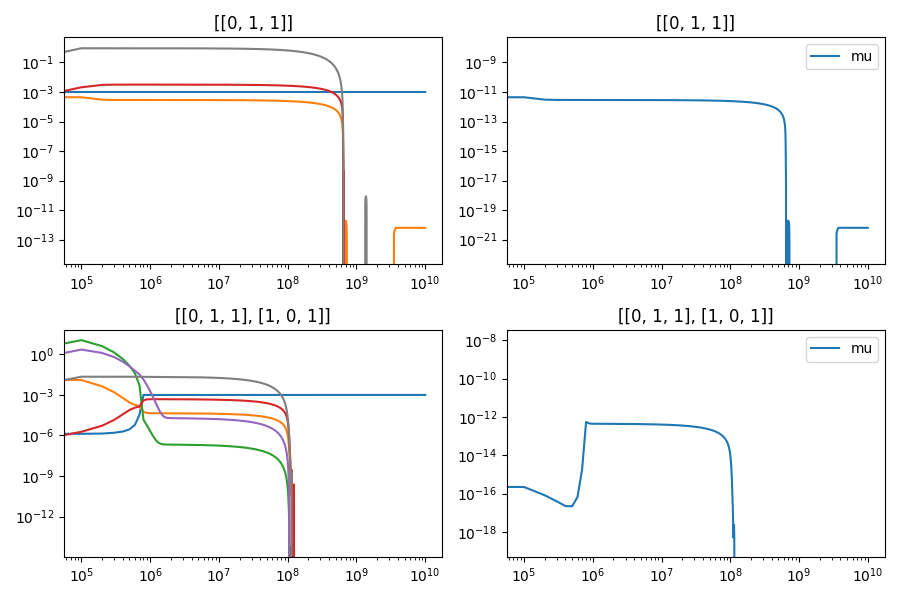
\includegraphics[width=10cm]{himeoka_timser_N2_M1_TMAX10_div7_NPLT5_Sext-3.png}
  \caption{$N=2,M=1,S_{\mathrm{ext}}=10^{-3}$とし,2通りの反応ネットワークについて時間発展を計算した結果.左は各成分濃度の時間発展(定常に至っているかの判定用なので,凡例は省略した.)であり,右は成長速度の時間発展である.}
  \label{fig:N2M1S-3}
\end{figure}

\begin{figure}[htbp]
  \centering
  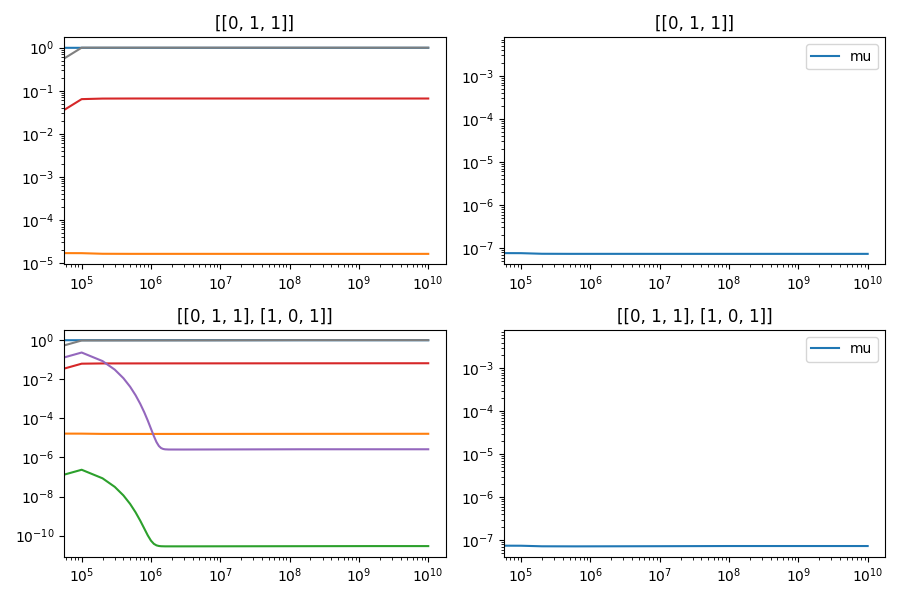
\includegraphics[width=10cm]{himeoka_timser_N2_M1_TMAX10_div7_NPLT5_Sext0.png}
  \caption{$N=2,M=1,S_{\mathrm{ext}}=10^{0}$とし,2通りの反応ネットワークについて時間発展を計算した結果.左は各成分濃度の時間発展(定常に至っているかの判定用なので,凡例は省略した.)であり,右は成長速度の時間発展である.}
  \label{fig:N2M1S0}
\end{figure}

\begin{figure}[htbp]
  \centering
  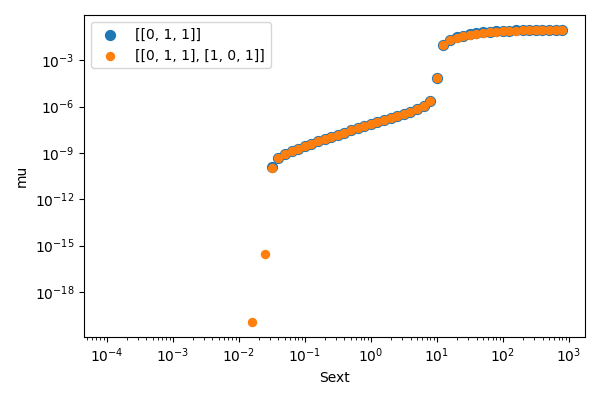
\includegraphics[width=10cm]{himeoka_trans_N2_M1_TMAX10_div7.png}
  \caption{$N=2,M=1$のときの,時刻$t=10^{10}$における2通りの反応ネットワークについての外部栄養濃度と成長速度の関係.刻み幅$dt=10^3$として計算した.}
  \label{fig:N2M1}
\end{figure}

\subsection{$N=3,M=1$の場合}
$N=3$の場合,$M=1,2$の両方がとれるが,ここでは$M=1$とした.
そして$p=0.3$として,ランダムに反応ネットワークを生成した.
まず$t=10^{9}$まで刻み幅$dt=10^3$で時間発展させると,$S_{\mathrm{ext}}=10^{-3}$のとき図\ref{fig:N3M1S-3},$S_{\mathrm{ext}}=10^{0}$のとき図\ref{fig:N3M1S1}が得られた.
これらから読み取れるように,$S_{\mathrm{ext}}= 10^{0}$のとき4番目の反応ネットの成分濃度が振動し,定常に至っていないという問題がある.
しかし,他の反応ネットは参考になると考え,時刻$t=10^9$における外部栄養濃度と成長速度の関係をプロットすると,図\ref{fig:N3M1}のようになった.
この図において,1番目の反応ネット$R=\{[0,1,1],[0,2,1],[1,0,1]\}$(と2番目の反応ネット$R=\{[0,1,1],[1,2,1]\}$)はおおよそ$N=2$の結果(図\ref{fig:N2M1})と同じ挙動を示していることが読み取れる.
一方で,3番目の反応ネット$R=\{[0,1,2]\}$は$S_{\mathrm{ext}}=10^3$でも生存していなかった.
また,4番目の反応ネット$R=\{[0,2,1],[1,0,2],[2,1,2]\}$は最大でも$\mu\approx 10^{-8}$程度の成長速度に留まっていた.

\begin{figure}[htbp]
  \centering
  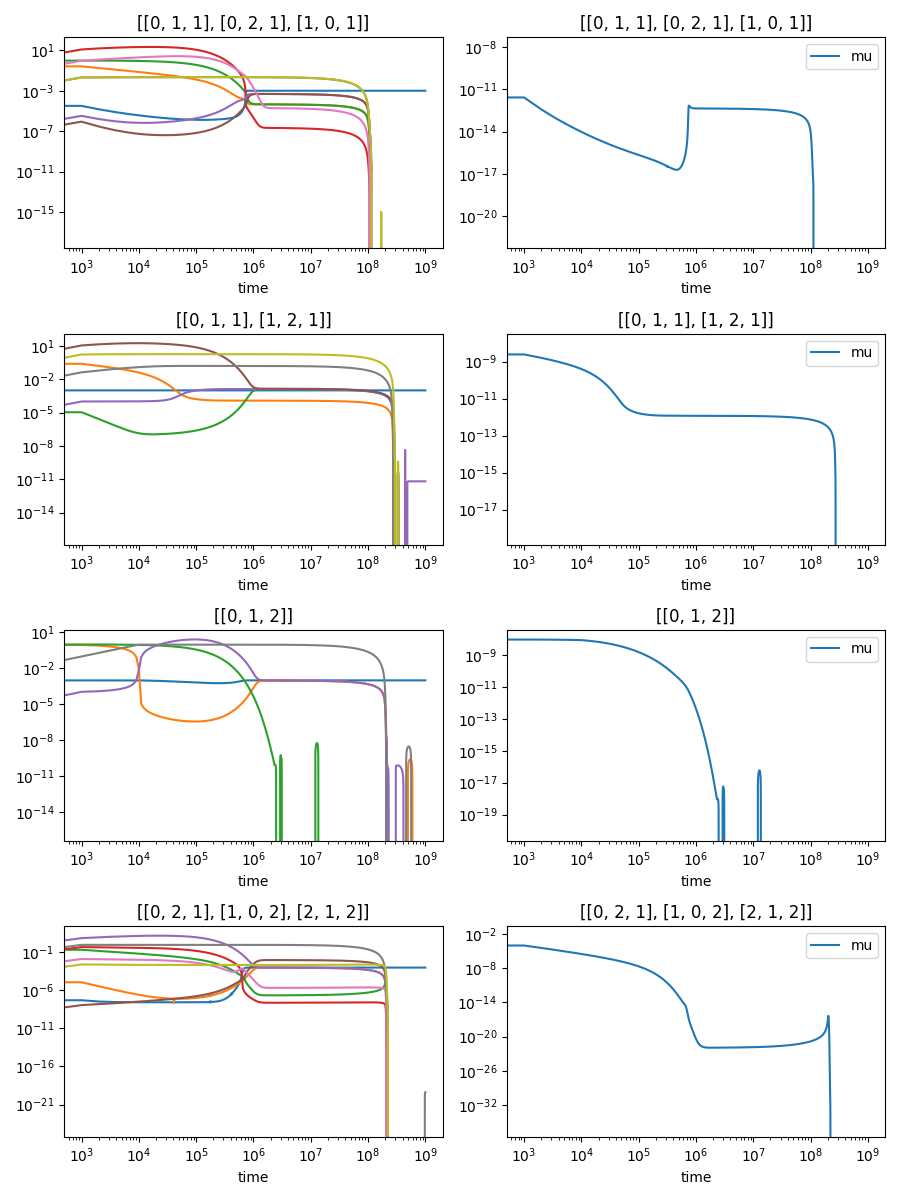
\includegraphics[width=10cm]{himeoka_timser_N3_M1_TMAX9_div6_NPLT5_Sext-3.png}
  \caption{$N=3,M=1,p=0.3,S_{\mathrm{ext}}=10^{-3}$とし,4通りのランダム反応ネットワークについて時間発展を計算した結果.刻み幅は$dt=10^3$とした.左は各成分濃度の時間発展(定常に至っているかの判定用なので,凡例は省略した.)であり,右は成長速度の時間発展である.}
  \label{fig:N3M1S-3}
\end{figure}

\begin{figure}[htbp]
  \centering
  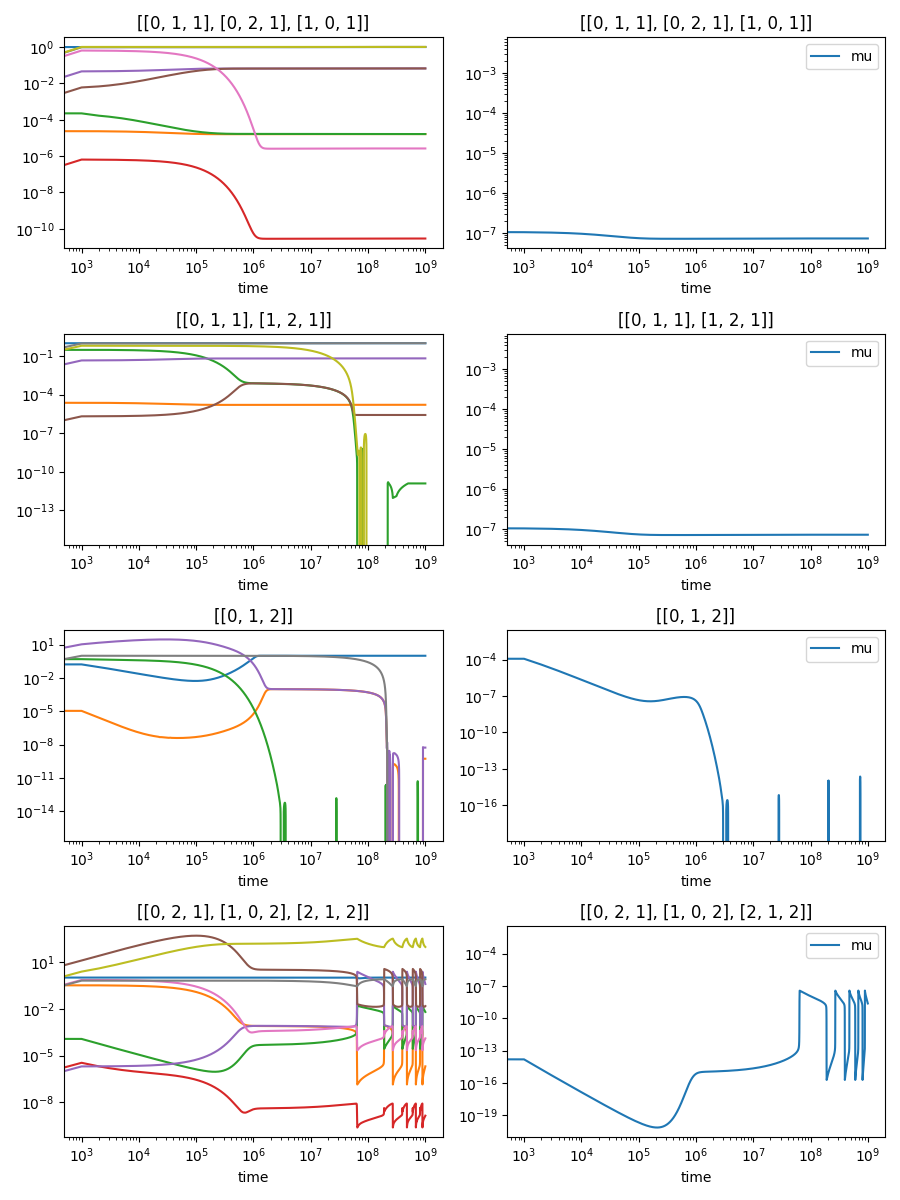
\includegraphics[width=10cm]{himeoka_timser_N3_M1_TMAX9_p3_div6_NPLT5_Sext0.png}
  \caption{$N=3,M=1,p=0.3,S_{\mathrm{ext}}=10^{0}$とし,4通りのランダム反応ネットワークについて時間発展を計算した結果.刻み幅は$dt=10^3$とした.左は各成分濃度の時間発展(定常に至っているかの判定用なので,凡例は省略した.)であり,右は成長速度の時間発展である.}
  \label{fig:N3M1S1}
\end{figure}

\begin{figure}[htbp]
  \centering
  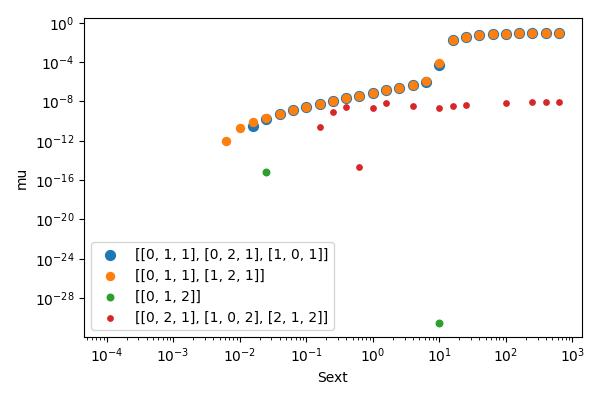
\includegraphics[width=10cm]{himeoka_trans_N3_M1_TMAX9_p3_div6.png}
  \caption{$N=3,M=1,p=0.3$のときの,時刻$t=10^9$における4通りのランダム反応ネットワークについての外部栄養濃度と成長速度の関係.刻み幅は$dt=10^3$とした.}
  \label{fig:N3M1}
\end{figure}

\section{考察}
今回試した計算では,転移点の位置のずれは有意な形では確認できなかった.
これは,転移点が確認できた反応ネットがオリジナルの姫岡モデルを包含している($[0,1,1]\in R$)からであると考える.
それ以外の反応ネットワークの転移点のずれについて議論するには,より多くのアンサンブルを取る必要があると考える.
というのも,$N=3,M=1$のときの計算結果から分かる通り,反応ネットによっては定常に至るまで長時間かかったり振動を続けたりするものがあり,こうした反応ネットでは転移を確認すること自体が難しいからである.
ここで,$N=3,M=1$の3番目の反応ネットが成長しないのは,成長と輸送に寄与する唯一の分子$x_1$を生成する反応の酵素$x_2$が決して新しく生成されないからであると説明できるが,4番目の反応ネットの振動現象については説明が思いつかなかった.
振動は刻み幅が大きすぎたことに由来するのではないかと考え,刻み幅$dt=10$として計算したが,同様の結果になった(図\ref{fig:oscil}).

\begin{figure}[htbp]
  \centering
  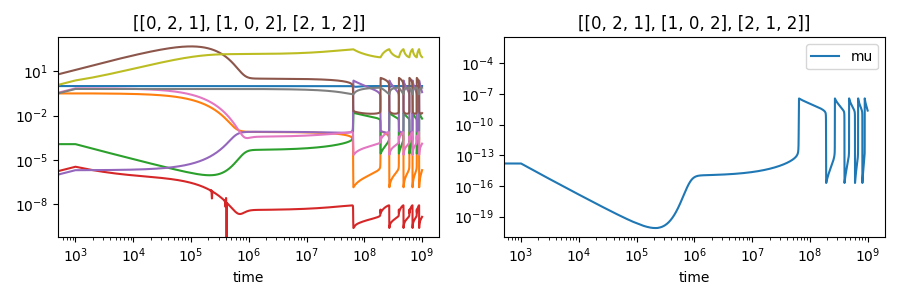
\includegraphics[width=10cm]{himeoka_timser_N3_M1_TMAX9_oscil_div8_NPLT6_Sext0.png}
  \caption{$N=3,M=1$の場合の計算に用いた振動してしまう反応ネット$R=\{ [0, 2, 1], [1, 0, 2], [2, 1, 2] \}$について,$S_{\mathrm{ext}}=10^{0}$とおいて刻み幅$dt=10$で時刻$t=10^9$まで時間発展を計算した結果.やはり振動が見られた.}
  \label{fig:oscil}
\end{figure}

一方で,二段階転移がうまくできている反応ネットは,どの濃度領域でも成長速度が他より大きかった.
そのため,進化計算を行ってそうした反応ネットを抽出すれば,姫岡モデルと同等の挙動が見られる可能性が高い.
このことは「進化によって生物の自由度が大幅に減少する」という研究\cite{furusawa}に対応しており,その結果到達する拘束条件として二段階転移が存在することを示唆している.

\begin{thebibliography}{99}
  \bibitem{himeoka} Himeoka, Y. and Kaneko, K. Theory for Transitions Between Exponential and Stationary Phases:
  Universal Laws for Lag Time. \textit{Phys. Rev. X.} \textbf{7}: 021049, 2017.  
  \bibitem{furusawa} Furusawa, C. and Kaneko, K. Formation of dominant mode by evolution in biological systems. \textit{Phys. Rev. E.} \textbf{97}: 042410, 2018.  
\end{thebibliography}

\end{document}